\documentclass[a4paper,UKenglish,cleveref, autoref]{lipics-v2019}
\usepackage{proof}
\usepackage{tikz}
\usepackage{gensymb}
\usepackage{enumitem}
\usepackage{booktabs}


\usetikzlibrary{automata,trees,calc,arrows.meta,positioning,decorations.pathreplacing,bending,shapes.geometric, intersections, hobby}



%This is a template for producing LIPIcs articles. 
%See lipics-manual.pdf for further information.
%for A4 paper format use option "a4paper", for US-letter use option "letterpaper"
%for british hyphenation rules use option "UKenglish", for american hyphenation rules use option "USenglish"
%for section-numbered lemmas etc., use "numberwithinsect"
%for enabling cleveref support, use "cleveref"
%for enabling cleveref support, use "autoref"


%\graphicspath{{./graphics/}}%helpful if your graphic files are in another directory

\bibliographystyle{plainurl}% the mandatory bibstyle

\title{Towards a Formalisation of Cook's Theorem} %TODO Please add

\titlerunning{}%optional, please use if title is longer than one line

\author{Lennard Gäher}{Saarland University, Germany}{s8legaeh@stud.uni-saarland.de}{}{}%TODO mandatory, please use full name; only 1 author per \author macro; first two parameters are mandatory, other parameters can be empty. Please provide at least the name of the affiliation and the country. The full address is optional

\authorrunning{L. Gäher}%TODO mandatory. First: Use abbreviated first/middle names. Second (only in severe cases): Use first author plus 'et al.'

\Copyright{Lennard Gäher}%TODO mandatory, please use full first names. LIPIcs license is "CC-BY";  http://creativecommons.org/licenses/by/3.0/

%\ccsdesc[100]{General and reference~General literature}
%\ccsdesc[100]{General and reference}%TODO mandatory: Please choose ACM 2012 classifications from https://dl.acm.org/ccs/ccs_flat.cfm 

%\keywords{Dummy keyword}%TODO mandatory; please add comma-separated list of keywords

%\category{}%optional, e.g. invited paper

\relatedversion{}%optional, e.g. full version hosted on arXiv, HAL, or other respository/website
%\relatedversion{A full version of the paper is available at \url{...}.}

\supplement{}%optional, e.g. related research data, source code, ... hosted on a repository like zenodo, figshare, GitHub, ...

%\funding{(Optional) general funding statement \dots}%optional, to capture a funding statement, which applies to all authors. Please enter author specific funding statements as fifth argument of the \author macro.


\nolinenumbers %uncomment to disable line numbering

\hideLIPIcs  %uncomment to remove references to LIPIcs series (logo, DOI, ...), e.g. when preparing a pre-final version to be uploaded to arXiv or another public repository

%Editor-only macros:: begin (do not touch as author)%%%%%%%%%%%%%%%%%%%%%%%%%%%%%%%%%%
\EventEditors{John Q. Open and Joan R. Access}
\EventNoEds{2}
\EventLongTitle{42nd Conference on Very Important Topics (CVIT 2016)}
\EventShortTitle{CVIT 2016}
\EventAcronym{CVIT}
\EventYear{2016}
\EventDate{December 24--27, 2016}
\EventLocation{Little Whinging, United Kingdom}
\EventLogo{}
\SeriesVolume{42}
\ArticleNo{23}
%%%%%%%%%%%%%%%%%%%%%%%%%%%%%%%%%%%%%%%%%%%%%%%%%%%%%%

\usepackage{gensymb}
\newcommand*{\listsofb}[1]{\mathcal{L} (#1)}
\newcommand*{\listsof}{\mathcal{L}~}

\newcommand{\None}{\emptyset}
\newcommand{\Some}[1]{\degree\kern-0.5ex#1}

\newcommand*{\match}{\textbf{match}~}
\newcommand*{\withl}{\textbf{[}~}
\newcommand*{\withr}{~\textbf{]}}
\newcommand*{\withm}{\quad\textbf{|}\quad}
\newcommand*{\llet}{\textbf{let}~}
\newcommand*{\lin}{\textbf{in}~}
\newcommand{\ITE}[3]{\textbf{if}~{#1}~\textbf{then}~{#2}~\textbf{else}~{#3}}

\newcommand{\Type}{\textsf{\bfseries T}}
\newcommand{\Prop}{\textsf{\bfseries P}}
\newcommand{\bool}{\textsf{B}}
\newcommand{\btrue}{\mathsf{T}}
\newcommand{\bfalse}{\mathsf{F}}
\newcommand{\andb}{\&\&}
\newcommand{\orb}{||}
\newcommand{\notb}{!}
\newcommand{\nat}{\mathsf{N}}
\newcommand{\natS}{1 + }
\newcommand{\length}[1]{|#1|}

\newcommand{\con}{\mathop{{+}\!\!\!{+}}}
\newcommand{\rev}{\mathsf{rev}}
\newcommand{\opt}[1]{\mathcal{O}{#1}}
\newcommand{\nil}{[]}

\newcommand{\eqb}[2]{#1\overset{?}{=}#2}

\newcommand{\bnfmid}{~\mid~}

\newcommand{\concat}{\con}


\newcommand{\TODO}[1]{\colorbox{red}{\LARGE TODO}:#1}

\newcommand{\strent}{\rightsquigarrow}
\newcommand{\constrent}{\overset{!}{\rightsquigarrow}}
\newcommand{\Rfinal}{R_{\text{final}}}

\newcommand{\bigO}[1]{\mathcal{O}{(#1)}}

\begin{document}

\maketitle

%TODO mandatory: add short abstract of the document
\begin{abstract}
  We present an outline of the planned proof of Cook's Theorem in Coq.
\end{abstract}

\newcommand{\gennp}{\textbf{GenNP}}
\newcommand{\strconrew}{\textbf{StrConRew}}
\newcommand{\binstrconrew}{\textbf{BinStrConRew}}
\newcommand{\csat}{\textbf{CSAT}}
\newcommand{\sat}{\textbf{SAT}}
\newcommand{\NP}{\textsf{NP}}

\newcolumntype{C}{>{$}c<{$}}
\newcommand{\rewwin}[2]{
  \begin{tabular}{C|C|C}
    #1 \\ 
    \midrule #2
  \end{tabular}
}

\newcommand{\blank}{\text{\textvisiblespace}}

\section{Introduction}
Cook's Theorem was proved in 1971 by Stephen A.\ Cook (and, in parallel, by Levin) and is one of the foundational results of computational complexity theory. 
It states that the satisfiability problem on CNFs \textbf{SAT} is NP-hard, that is, any problem $Q \in NP$ can be polynomial-time reduced to it: $Q \prec_{\text{p}} \textbf{SAT}$. 
There are multiple well-known textbook proofs available. We strive to adapt a particularly simple one which encodes the transitions of a Turing machine using logical formulas layed out in a tableau.
An outline of this classical proof can be found in~\cite{Sipser:TheoryofComputation}. 

Despite the conceptual simplicity of the original proof, the formalisation is quite demanding. The key difficulties lie with 
\begin{itemize}
  \item encoding nondeterminism, 
  \item working with our particular representation of Turing machine tapes,
  \item reserving enough space for the Turing machine beforehand since the logical formula must have a fixed size,
  \item ensuring time bounds.
\end{itemize}

Our reduction has the following structure: 
\begin{center}
  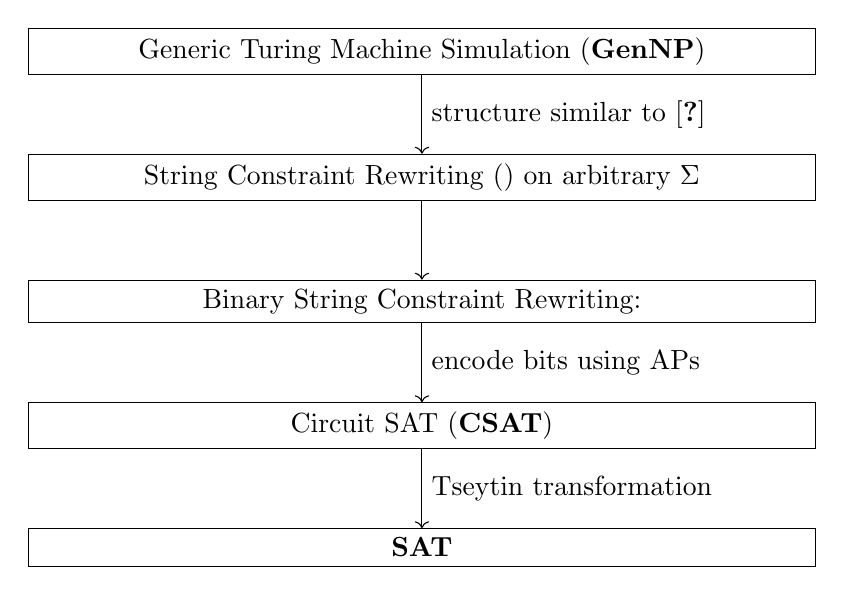
\begin{tikzpicture}
    \node[rectangle, draw=black, minimum width = 10cm] (gennp) {Generic Turing Machine Simulation (\textbf{GenNP})};
    \node[rectangle, draw=black, below = of gennp, minimum width = 10cm] (strrew1) {String Constraint Rewriting (\strconrew) on arbitrary $\Sigma$};
    \node[rectangle, draw=black, below = of strrew1, minimum width = 10cm] (strrew2) {Binary String Constraint Rewriting: \binstrconrew};
    \node[rectangle, draw=black, below = of strrew2, minimum width = 10cm] (csat) {Circuit SAT (\textbf{CSAT})};
    \node[rectangle, draw=black, below = of csat, minimum width = 10cm] (sat) {\textbf{SAT}};
    \draw[->] 
      (gennp) edge node[right] {structure similar to~\cite{Sipser:TheoryofComputation}} (strrew1)
      (strrew1) edge (strrew2)
      (strrew2) edge node[right] {encode bits using APs} (csat)
      (csat) edge node[right] {Tseytin transformation} (sat);
  \end{tikzpicture}
\end{center}

The reduction from \gennp{} to \strconrew{} does the main job of encoding the behaviour of Turing machines. We are then left with a structurally much simpler problem on strings. 
In order to be able to encode this problem using logical formulas, we then simplify the alphabet to $\{0, 1\}$ in a reduction to \binstrconrew, making it possible to encode single characters using a boolean-valued atomic proposition in the reduction to \csat. The encoding of the string rewriting system that we use will not be in conjunctive normal form (CNF), therefore we then use the Tseytin transformation in a reduction from \csat{} to \sat{} on CNFs. 

\section{Involved Languages}
We first give a formal description of the involved problems. 

\subsection*{Generic Turing Machine Simulation (\gennp{})}
The formalisation of Turing machines we use has been introduced in~\cite{ForsterEtAl:2019:VerifiedTMs}, although we do not have any use for the abstractions developed for the programming of Turing machines in Coq. This formalisation is based on one originally done in the proof assistant Matita~\cite{Asperti2015AFO}. 

For the representation of tapes, no blank symbol is explicitly specified. Instead, the constructors explicitly specify whether the head is currently at the left or the right end of the used tape area.
\begin{definition}[Tapes] \label{def:tapes}
  Let $\Sigma$ be a type. A tape is defined by
  \[\textsf{Tape}_\Sigma ::= \textsf{niltape} \bnfmid \textsf{leftof}~r~rs \bnfmid \textsf{midtape}~ls~m~rs \bnfmid \textsf{rightof}~l~ls \]
  with $l, m, r : \Sigma$ and $rs, ls : \listsof{\Sigma}$. 
\end{definition}

For each possible tape state and head position, this admits a unique representation: $\textsf{niltape}$ specifies that the tape is completely empty, $\textsf{midtape}~ls~m~rs$ is used when the head currently resides on the symbol $m$ and there are possibly further symbols to the left ($ls$) or right ($rs$). $\textsf{leftof}$ and $\textsf{rightof}$ indicate that the head is currently one symbol to the left or right of the already used tape $l::ls$ or $r::rs$, respectively. 
$ls$ and $rs$ are ordered such that the symbol closest to the head is at the head of the list. 

\begin{definition}[Turing machines]
  An $n$-tape Turing machine $M : \textsf{TM}_\Sigma^n$ over a finite alphabet $\Sigma$ is a tuple $M = (Q, \delta, \mathit{start}, \mathit{halt})$, where $Q$ is the finite type of states, $\delta : Q \times {(\opt{(\Sigma)})}^n \rightarrow Q \times {(\textsf{Act}_\Sigma)}^n$ (with actions $\textsf{Act}_\Sigma := \opt{(\Sigma)} \times \textsf{Move}$ and $\textsf{Move} ::= L \bnfmid R \bnfmid N$) is the transition function, $\mathit{start} : Q$ is the initial state and $\mathit{halt} : Q \rightarrow \bool$ represents the halting states. 
\end{definition}

We now give the basics of the semantics of Turing machines. Let us fix an alphabet $\Sigma$ and a $n$-tape Turing machine $M$.
A single action of the Turing machine on a tape is executed by the function $\textsf{doAct} : \textsf{Tape}_\Sigma \rightarrow \textsf{Act} \rightarrow \textsf{Tape}_\Sigma$, the definition of which can be found in the appendix. This can be extended canonically to a function $\textsf{doAct}$ acting on a vector of tapes.

Configurations of the Turing machine $M$ are defined as pairs of a state and a vector of tapes: $\textsf{Conf}_M : Q \times {(\textsf{Tape}_\Sigma)}^n$. One computational step of $M$ is then executed by the function $\textsf{step}_M : \textsf{Conf}_M \rightarrow \textsf{Conf}_M$. We will denote the induced relation on configurations by $c_1 \succ c_2$.

The function $\textsf{loop}_M : \textsf{Conf}_M \rightarrow \nat \rightarrow \opt{\textsf{Conf}_M}$ can then be used to simulate $M$ for a given number of steps. If the Turing machine halts, starting from $c_1$, in a halting configuration $c_2$ within this number of steps, written $c_1 \rhd c_2$, it returns $c_2$, otherwise it returns $\None$.


\begin{definition}[\gennp{}]
  Given a deterministic 1-tape Turing machine $M$ and numbers $k$ and $t$, decide whether there is an input $x$ of length $\length{x} \le k$ such that $M$ halts on $x$ in at most $t$ steps: $ \exists c, (\mathit{halt}, x) \succ^{\le t} c $
\end{definition}

A more wide-spread (but equivalent) definition of a generic problem for Turing machines is the following: Given a nondeterministic Turing machine $M$ and an input $x$ and a number $t$, decide whether $M$ halts on $x$ in at most $t$ steps. 
We do not use this variant since it would require us to formalise the notion of nondeterminism. Instead, our definition builds on the well-known verifier characterisation of \NP{}. The whole input of the Turing machine is regarded as a certificate; the instance itself can be statically encoded in the states of the Turing machine.

The restriction to 1-tape Turing machines is without loss of generality, a fact which has also been formalised in Coq~\cite{ForsterEtAl:2019:VerifiedTMs}. 

Using a classical definition of the complexity class \NP{} using Turing machines, one is easily convinced that \gennp{} is \NP{}-hard. For our definition using the call-by-value $\lambda$-calculus L, this isn't straightforward at all, though. We thus leave the problem of proving the \NP{}-hardness of \gennp{} open for now, but remark on this problem in Section~\ref{TODO}.

\subsection*{String Constraint Rewriting (\strconrew{})}
This problem works on strings of a fixed length $l$ over an alphabet $\Sigma$. Starting with an initial string $x_0$, the task is to determine whether there is a sequence of strings $x_1, \ldots, x_t$ such that $x_{i+1}$ validly follows from $x_i$, denoted by $x_i \strent x_{i+1}$, such that $x_t$ satisfies a final condition. The number $t$ is fixed. All of the strings in the sequence must have the same length $l$. The relation $x_i \strent x_{i+1}$ is described by a set $R$ of rewrite windows.

Each window specifies a rewrite $a \constrent b$ for strings $a, b$ of a fixed length $w \le l$. Basically, in order for $x_i \strent x_{i+1}$ to hold, each of the characters of $x_{i+1}$ must be derived from $x_i$ using a rewrite window.
More precisely, in order for a string $x_{i+1}$ to validly follow from a string $x_i$, for each offset $j \cdot o$ in $x_i$ which is a multiple of a rewriting offset $o$, a rewrite window must hold:
\[\bigwedge_{0 \le j\cdot o \le l - w + 1} \bigvee_{(a \constrent b) \in R} (x_i[j\cdot o..j\cdot o+w-1] = a \land x_{i+1}[j\cdot o..j\cdot o+w-1] = b) \]

The final condition is given by a set of substring constraints $\Rfinal$: In order for the final string $x_t$ to be valid, there needs to be $x \in \Rfinal$ such that $x$ is a substring of $x_t$:
\[\bigvee_{x \in \Rfinal} \bigvee_{0 \le j \le l - \length{x} + 1} (x_t[j..j+\length{x} -1] = x) \]

\newcommand*{\validR}{\textsf{valid}}

\begin{example}[Generating permutations]
  In this example, we develop an instance of \strconrew{} that determines whether $aaabc$ is a permutation of $abaca$ which can be obtained with at most 10 transpositions. 

  We work over the alphabet $\Sigma = \{a, b, c\}$ and a string length of $5$. We start with the initial string $x_0=abaca$ and our final substring constraint is $\{aaabc\}$; that is, we require that $aaabc$ is a substring of the final string, which implies equality because the final string will have a length of $5$.

  Our rewrite windows have a width of 3 characters and we use an offset $o =1$. They allow for exchanging two adjacent characters and thus each rewrite step will capture . Namely, we have the following rewrite windows where $\sigma$ ranges over $\Sigma$:
  \TODO{more suitable example where the limit in the number of steps has a meaning}
\end{example}
    
We now formally define \strconrew{}:
\begin{definition}\label{def:strconrew}
  Given: 
  \begin{itemize}
    \item an alphabet $\Sigma$
    \item a string length $l$,
    \item a step count $t$,
    \item an initial string $x_0 \in \Sigma^l$,
    \item a width $w$ of rewrite windows, 
    \item a rewriting offset $o$
    \item a list of rewrite windows $R = \{a_i \constrent b_i | i \in \nat \land a_i, b_i \in \Sigma^w\}$,
    \item a set of final substring constraints $\Rfinal = \{f_i | i \in \nat \land \exists k \le l, f_i \in \Sigma^k\}$
  \end{itemize}

  Determine if there is a sequence of strings $x_1, \ldots, x_t \in \Sigma^l$ such that 
  \begin{itemize}
    \item For every $0 \le i < t$ it holds that $\validR(x_i, x_{i+1})$, where $\validR$ is defined as follows:
      \[\forall (0 \le j\cdot o \le l -w + 1), \exists (a \constrent b) \in R, x_i[j\cdot o..j\cdot o+ k-1] = a \land x_{i+1}[j\cdot o..j\cdot o+k-1] = b \]
    \item There exists an $x \in \Rfinal$ such that $x$ is a substring of $x_t$, i.e.\ there is $0 \le j \le l - \length{x} + 1$ with $x = x_t[j..j+\length{x} - 1]$.
  \end{itemize}
\end{definition}

We admit that this definition is quite complex, but hope that the reason for this complexity becomes clear in the reduction from \gennp{}.

Finally, we establish a few properties about \strconrew{}. For the remainder of this section, fix a rewriting system with parameters according to Definition~\ref{def:strconrew}.

\begin{lemma}\label{lem:rewind}
  $a :: b :: c :: rs \strent{} a' :: b' :: c' :: rs'$ iff $b :: c :: rs \strent{} b' :: c' :: rs'$ and $abc \constrent{} a'b'c'$. 
\end{lemma}
This lemma enables us to prove rewrites inductively.

\section{Reducing \gennp{} to \strconrew{}}
The basic idea of this reduction is very similar to the reduction in~\cite{Sipser:TheoryofComputation}, although we encode Turing machines using a constrained string rewriting system instead of logical formulas. We defer the handling of nondeterministically ``guessing'' an input of size at most $k$ to Section~\ref{TODO} and instead first deal with a setting in which we are given a deterministic 1-tape Turing machine and a fixed input $\sigma_1, \ldots, \sigma_k$ of size $k$. 

\subsection{Encoding Deterministic Turing Machines}
The configurations of the Turing machine are laid out in a tableau of $t \cdot (1 + 2(k + t + 2))$ characters. Each configuration is modelled by one line of the tableau, that is, a string of length $1 + 2(k + t + 2)$. Starting from an initial configuration $x_0$, the transition function is then encoded using rewrite windows of width 3 and rewriting offset 1. The final constraint is that the final configuration contains the symbol of a halting state. 
Using the string rewriting problem, it is then determined whether there exists an execution of the Turing machine for which it halts after at most $t$ steps. 

\begin{center}
  \begin{tikzpicture}
    \draw (1.5, -4) -- (1.5, 3) -- (10, 3) -- (10, -4) -- (1.5, -4);
    \draw (2, -4) -- (2, 3);
    \draw (2.5, 3) -- (2.5, 2);
    \draw (9.5, -4) -- (9.5, 3);
    \draw (1.5, 2.5) -- (10, 2.5);
    \draw (1.5, -3.5) -- (10, -3.5);
    \draw (1.5, 2) -- (10, 2);
    \draw (1.5, 1.5) -- (2, 1.5);
    \draw (9.5, 1.5) -- (10, 1.5);

    \draw (4.5, 3) -- (4.5, 2);
    \draw (5, 3) -- (5, 2);
    \draw (5.5, 3) -- (5.5, 2);
    \draw (6, 3) -- (6, 2);
    \draw (7, 3) -- (7, 2);
    \draw (7.5, 3) -- (7.5, 2);
    \draw (8, 3) -- (8, 2);
    \draw (9, 3) -- (9, 2);
    %\draw (2.5, 3) -- (2.5, 2);
    %\draw (3, 3) -- (3, 2.5);
    %\draw (4.5, 3) -- (4.5, 2.5);
    %\draw (5, 3) -- (5, 2.5);
    %\draw (5.5, 3) -- (5.5, 2.5);
    %\draw (7.5, 3) -- (7.5, 2.5);

    \node at (1.75, 2.75) {\blank};
    \node at (1.75, 2.25) {\blank};
    \node at (1.75, 1.75) {\blank};
    %\node at (1.75, -3.75) {\blank};
    \node at (9.75, 2.75) {\blank};
    \node at (9.75, 2.25) {\blank};
    \node at (9.75, 1.75) {\blank};
    %\node at (9.75, -3.75) {\blank};

    \node at (2.25, 2.75) {\textvisiblespace};
    \node at (3.5, 2.75) {$\ldots$};
    \node at (4.75, 2.75) {\textvisiblespace};
    \node at (5.25, 2.75) {\small $q_0^{\sigma_1}$};
    \node at (5.75, 2.75) {\small $\sigma_2$};
    \node at (6.5, 2.75) {$\ldots$};
    \node at (7.25, 2.75) {\small $\sigma_k$};
    \node at (7.75, 2.75) {\textvisiblespace};
    \node at (8.5, 2.75) {$\ldots$};
    \node at (9.25, 2.75) {\textvisiblespace};

    %\node at (6.5, 2.75) {$\ldots$};
    %\node at (5, 2.25) {$\ldots$};

    \node at (1.75, -0.375) {$\vdots$};
    \node at (9.75, -0.375) {$\vdots$};

    \draw (4, -0.5) -- (4, 0.5) -- (5.5, 0.5) -- (5.5, -0.5) -- (4, -0.5);
    \draw (4.5, -0.5) -- (4.5, 0.5);
    \draw (5, -0.5) -- (5, 0.5);
    \draw (4, 0) -- (5.5, 0);

    \path[<->] (1, -4) edge node[fill=white, anchor=center, pos= 0.5] {\small t} (1, 3);
    \path[<->] (1.5, -4.5) edge node[fill=white, anchor=center, pos=0.5] {\small $2 (k + t + 2) + 1$} (10, -4.5);
    \path[<->] (5.5, 3.5) edge node[fill=white, anchor=center, pos=0.5] {\small $k-1$} (7.5, 3.5);

    \node at (11, 2.75) {\small 1\textsuperscript{st} config};
    \node at (11, 2.25) {\small 2\textsuperscript{nd} config};
    \node at (11, 1.75) {\small 3\textsuperscript{rd} config};
  \end{tikzpicture}
\end{center}

In contrast to the representation of tapes in Definition~\ref{def:tapes}, we cannot make the string size grow dynamically, but instead have to make sure to allocate enough space such that the Turing machine will never run out of space during its $t$ computation steps. Turing machines can, in $t$ steps of computation, only visit $t+1$ cells. Since our tapes are two-sided, we reserve space for $2(k + t + 2)+1$ cells ($k + t + 2$ cells in each direction\footnote{We need $k+t$ cells because the Turing machine might never visit the input cells; the additional 2 cells are there in order to make reasoning easier.}, i.e.\ left and right, and one cell on which the head resides initially).
In general, most of these cells will be unused. We therefore introduce explicit blanks \blank{} which are used for these unused cells.

For the encoding of configurations, we directly follow the representation of tapes of Definition~\ref{def:tapes}.
At the center of the string, there is always a symbol $q^m$ encoding the current state $q$ and the symbol $m$ the head currently resides on (this symbol may also be a blank \blank{} if the tape is empty or the head resides left or right of the used tape region). 
To the left of the center symbol, there will be the encoded left part of the tape, and to the right will be the encoded right part of the tape. 

\newcommand{\polneg}[1]{\overleftarrow{#1}}
\newcommand{\polpos}[1]{\overrightarrow{#1}}
\newcommand{\polneut}[1]{\overline{#1}}
\subsubsection{Encoding: High-Level Details}\label{sec:rewrules}
In this section we describe more high-level details of encoding the states, alphabet and the transition function using rewrite windows of width 3. 

We desire that the following properties hold for our encoding:
\begin{enumerate}
  \item the alphabet size and space usage are reasonable and allow for a polynomial-time reduction,
  \item for every given representation of tapes according to Definition~\ref{def:tapes}, there is a unique encoding, and vice-versa,
  \item each transition of the Turing machine can be done using one step of the rewriting system, and
  \item the simulation is sound and complete.
\end{enumerate}
All of these properties are reasonable to desire in order to be able to obtain intuitive proofs.
Our encoding will satisfy properties (1), (3) and (4); (2) will be nearly satisfied, with a small degree of freedom in the encoding.

The main difficulty with encoding the transitions lies with our representation of tapes. Since the tape representation doesn't include an explicit blank symbol but our encoding needs to rely on blanks in order to be able to preallocate all the needed space statically, we have to work around this incompatibility. We will thus use symbols $q^m$ for the current state and current symbol under the head. 
Actually, the head position will be fixed: A symbol $q^m$ will always be placed at the center of the string. The \emph{tape contents} are moved around it. This is necessary in order to fulfill property (2): Otherwise, there would be $\bigO{t}$ many different representations for each configuration since we could arbitrarily shift around the state and the tape contents inside the string.
This invariant also makes proofs easier: We always know that a state character can only appear at the center of the string and nowhere else.

We now define the alphabet.
Let $\Sigma$ be the finite type representing the Turing machine $M$'s alphabet and $Q$ the finite type of states. The alphabet $\Gamma$ for the string rewriting problem then is 
\begin{align*}
  \Sigma' := \{\polneg{\sigma}, \polpos{\sigma}, \polneut{\sigma} | \sigma \in \Sigma\} \\
  \Gamma := \{\blank\} \cup \{q^m | q \in Q, m \in \Sigma \cup \{\blank\}\} \cup \Sigma'. 
\end{align*}
As mentioned above, the blank \blank{} is written in cells currently not in use by $M$. Symbols of the form $q^m$ are pairs of the current state and the symbol currently under $M$'s head and will always reside at the center of the string.
Finally, symbols $\omega \in \Sigma'$ are used for ordinary elements of $M$'s tape. Each of these symbols is annotated with a polarity $p \in \{-1, 0, 1\}$ which annotates the last head movement (its sense will become clear when dealing with the transition function). We say that $\polneg{\sigma}$ has a \emph{negative} (or \emph{left}) polarity, $\polneut{\sigma}$ is \emph{neutral} and $\polpos{\sigma}$ has a \emph{positive} (or \emph{right}) polarity\footnote{At this point I wondered about this common connotation of ``left'' $\eqsim$ ``negative'' and ``right'' $\eqsim$ ``positive''. Apparently it's all down to left-handedness and right-handedness, historically.}. 

The key idea now is to use rewrite windows with a width of 3, just as in the original reduction~\cite{Sipser:TheoryofComputation}. Also remember that we are using an offset of 1. Thus, one of the windows has to hold at every offset of a configuration. 

\begin{example}
  \TODO{some example of a Turing machine and the execution of a transition}
\end{example}


In the following, the letter $\sigma$ will range over $\Sigma$, $m$ will range over $\Sigma \cup \{\blank\}$. 
We will also use $\sigma$ to refer to elements of $\Sigma'$ when we do not care about the polarity, and will use polarities with elements $m \in \Sigma'$, e.g.\ $\polpos{m}$; in case that $m \in \Sigma$, this has the usual effect, while the polarity can be ignored if $m = \blank$. 


The following windows are created for moving the tape. For the moment, the annotations stating to which half of the configuration string they can be applied can be disregarded.
\paragraph*{Move Tape Right}
\begin{center}
  \rewwin{\sigma_1 & \sigma_2 & \sigma_3}{\polpos{\sigma_4} & \polpos{\sigma_1} & \polpos{\sigma_2}}
  \rewwin{\sigma_1 & \sigma_2 & m_1}{\polpos{\sigma_3} & \polpos{\sigma_1} & \polpos{\sigma_2}}  
  \quad (both halves)
  \\[3ex]
  \rewwin{\sigma_1 & \blank & \blank}{\polpos{\sigma_2} & \polpos{\sigma_1} & \blank}
  \rewwin{\blank & \blank & \blank}{\polpos{\sigma_1} & \blank & \blank} 
  \quad (right half)
\end{center}

\paragraph*{Move Tape Left}
\begin{center}
  \rewwin{\blank & \blank & \blank}{\blank & \blank & \polneg{\sigma_1}}
  \rewwin{\blank & \blank & \sigma_1}{\blank & \polneg{\sigma_1} & \polneg{\sigma_2}} 
  \quad{(left half)} \\[3ex]
  \rewwin{m_1 & \sigma_1 & \sigma_2}{\polneg{\sigma_1} & \polneg{\sigma_2} & \polneg{\sigma_3}}
  \rewwin{\sigma_1 & \sigma_2 & \sigma_3}{\polneg{\sigma_2} & \polneg{\sigma_3} & \polneg{\sigma_4}}
  \quad{(both halves)} \\[3ex]
\end{center}

\paragraph*{Identity}
\begin{center}
  \rewwin{\blank & \blank & \blank}{\blank & \blank & \blank} 
  \rewwin{\sigma_1 & \sigma_2 & \sigma_3}{\polneut{\sigma_1} & \polneut{\sigma_2} & \polneut{\sigma_3}}
  \quad{(both halves)}\\[3ex]
  \rewwin{\blank & \blank & \sigma_1}{\blank & \blank & \polneut{\sigma_1}}
  \rewwin{\blank & \sigma_1 & \sigma_2}{\blank & \polneut{\sigma_1} & \polneut{\sigma_2}}
  \quad{(left half)} \\[3ex]
  \rewwin{\sigma_1 & \sigma_2 & \blank}{\polneut{\sigma_1} & \polneut{\sigma_2} & \blank}
  \rewwin{\sigma_1 & \blank & \blank}{\polneut{\sigma_1} & \blank & \blank}
  \quad{(right half)}
\end{center}

Note that many of the rules are symmetric since we need left and right versions for most of them. 
Also note that these rules explicitly encode the invariant that all elements of $M$'s tape are stored contiguously, without any blanks \blank{} in between.

\paragraph*{Transitions}

For every entry of the transition function, we introduce the following windows. Note that, when moving the head left, we have to shift the tape right, and we have to shift the tape left, if the head is moving right.

\paragraph*{$\delta(q, \Some{a}) = (p, \Some{b}, \textsf{L})$:}
\begin{center}
  \rewwin{\blank & q^a & m_1}{\blank & p^\blank & \polpos{b}}
  \rewwin{\sigma_1 & q^a & m_1}{\polpos{m_2} & p^{\sigma_1} & \polpos{b}} \\[3ex]
  \rewwin{\blank & \blank & q^a}{\blank & \blank & p^\blank} 
  \rewwin{\blank & \sigma_1 & q^a}{\blank & \blank & p^{\sigma_1}}
  \rewwin{\sigma_1 & \sigma_2 & q^a}{\polpos{m_1} & \polpos{\sigma_1} & p^{\sigma_2}} \\[3ex]
  \rewwin{q^a & \blank & \blank}{p^{m_1} & \polpos{b} & \blank}
  \rewwin{q^a & \sigma_1 & m_1}{p^{m_2} & \polpos{b} & \polpos{\sigma_1}}
\end{center}

\paragraph*{$\delta(q, \Some{a}) = (p, \Some{b}, \textsf{R})$:}
\begin{center}
  \rewwin{m_1 & q^a & \blank}{\polneg{b} & p^{\blank} & \blank}
  \rewwin{m_1 & q^a & \sigma_1}{\polneg{b} & p^{\sigma_1} & \polneg{m_2}} \\[3ex]
  \rewwin{q^a & \blank & \blank}{p^{\blank} & \blank & \blank}
  \rewwin{q^a & \sigma_1 & \blank}{p^{\sigma_1} & \blank & \blank}
  \rewwin{q^a & \sigma_1 & \sigma_2}{p^{\sigma_1} & \polneg{\sigma_2} & \polneg{m_1}} \\[3ex]
  \rewwin{\blank & \blank & q^a}{\blank & \polneg{b} & p^{m_1}}
  \rewwin{m_1 & \sigma_1 & q^a}{\polneg{\sigma_1} & \polneg{b} & p^{m_2}}
\end{center}

\paragraph*{$\delta(q, \Some{a}) = (p, \Some{b}, \textsf{N})$:}
\begin{center}
  \rewwin{m_1 & q^a & m_2}{\polneut{m_1} & p^b & \polneut{m_2}} \\[3ex]
  \rewwin{q^a & \sigma_1 & m_1}{p^b & \polneut{\sigma_1} & \polneut{m_1}}
  \rewwin{q^a & \blank & \blank}{p^b & \blank & \blank} \\[3ex]
  \rewwin{m_1 & \sigma_1  & q^a}{\polneut{m_1} & \polneut{\sigma_1} & p^b} 
  \rewwin{\blank & \blank & q^a}{\blank & \blank & p^b}
\end{center}

\paragraph*{$\delta(q, \Some{a}) = (p, \None, \textsf{L})$:}
\begin{center}
  \rewwin{\blank & q^a & m_1}{\blank & p^\blank & \polpos{a}}
  \rewwin{\sigma_1 & q^a & m_1}{\polpos{m_2} & p^{\sigma_1} & \polpos{a}} \\[3ex]
  \rewwin{\blank & \blank & q^a}{\blank & \blank & p^\blank} 
  \rewwin{\blank & \sigma_1 & q^a}{\blank & \blank & p^{\sigma_1}}
  \rewwin{\sigma_1 & \sigma_2 & q^a}{\polpos{m_1} & \polpos{\sigma_1} & p^{\sigma_2}} \\[3ex]
  \rewwin{q^a & \blank & \blank}{p^{m_1} & \polpos{a} & \blank}
  \rewwin{q^a & \sigma_1 & m_1}{p^{m_2} & \polpos{a} & \polpos{\sigma_1}}
\end{center}

The rules for $\delta(q, \Some{a}) = (p, \None, \textsf{R})$ and $\delta(q, \Some{a}) = (p, \None, \textsf{N})$ can be derived from the $\Some{b}$ cases in a similar fashion and can be found in the appendix.

For the cases where the current symbol is a blank, it must hold that there is a blank to the left or to the right (otherwise the invariant that all of the used cells are contiguous would be violated).
\paragraph*{$\delta(q, \None) = (p, \Some{b}, \textsf{L})$:}
\begin{center}
  \rewwin{\blank & q^\blank & m_1}{\blank & p^\blank & \polpos{b}} 
  \rewwin{\sigma_1 & q^\blank & \blank}{\polpos{m_1} & q^{\sigma_1} & \polpos{b}} \\[3ex]
  \rewwin{\sigma_1 & \sigma_2 & q^\blank}{\polpos{m_1} & \polpos{\sigma_1} & p^{\sigma_2}}
  \rewwin{\blank & \sigma_1 & q^{\blank}}{\blank & \blank & p^{\sigma_1}}
  \rewwin{\blank & \blank & q^\blank}{\blank & \blank & p^\blank} \\[3ex]
  \rewwin{q^\blank & \sigma_1 & m_1}{q^{m_2} & \polpos{b} & \polpos{\sigma_1}}
  \rewwin{q^\blank & \blank & \blank}{q^{m_1} & \polpos{b} & \blank}
\end{center}

\paragraph*{$\delta(q, \None) = (p, \Some{b}, \textsf{N})$:}
\begin{center}
  \rewwin{m_1 & q^\blank & \blank}{\polneut{m_1} & q^b & \blank}
  \rewwin{\blank & q^\blank & m_1}{\blank & q^b & \polneut{m_1}} \\[3ex]
  \rewwin{m_1 & \sigma_1 & q^\blank}{\polneut{m_1} & \polneut{\sigma_1} & q^b}
  \rewwin{\blank & \blank & q^{\blank}}{\blank & \blank & q^b} \\[3ex]
  \rewwin{q^{\blank} & \sigma_1 & m_1}{q^b & \polneut{\sigma_1} & \polneut{m_1}} 
  \rewwin{q^\blank & \blank & \blank}{q^b & \blank & \blank}
\end{center}

\paragraph*{$\delta(q, \None) = (p, \Some{b}, \textsf{R})$:}
\begin{center}
  \rewwin{m_1 & q^\blank & \blank}{\polneg{b} & p^\blank & \blank} 
  \rewwin{\blank & q^\blank & \sigma_1}{\polneg{b} & p^{\sigma_1} & \polneg{m_1}} \\[3ex]
  \rewwin{q^\blank & \sigma_1 & \sigma_2}{p^{\sigma_1} & \polneg{\sigma_2} & \polneg{m_1}} 
  \rewwin{q^\blank & \sigma_1 & \blank}{p^{\sigma_1} & \blank & \blank} 
  \rewwin{q^\blank & \blank & \blank}{p^\blank & \blank & \blank} \\[3ex]
  \rewwin{m_1 & \sigma_1 & q^\blank}{\polneg{\sigma_1} & \polneg{b} & q^{m_2}}
  \rewwin{\blank & \blank & q^\blank}{\blank & \polneg{b} & q^{m_2}}
\end{center}

If the head is currently on a blank (i.e.\ the head is beyond the currently used tape region), the tape is not moved if again a blank is written, meaning that no new cell is required.
\paragraph*{$\delta(q, \None) = (p, \None, \textsf{L})$:}
\begin{center}
  \rewwin{\blank & q^\blank & m_1}{\blank & p^\blank & \polneut{m_1}} 
  \rewwin{\sigma_1 & q^\blank & \blank}{\polpos{m_1} & p^{\sigma_1} & \blank} \\[3ex]
  \rewwin{\blank & \blank & q^\blank}{\blank & \blank & p^\blank}
  \rewwin{\blank & \sigma_1 & q^\blank}{\blank & \blank & q^{\sigma_1}}
  \rewwin{\sigma_2 & \sigma_1 & q^\blank}{\polpos{m_1} & \polpos{\sigma_2} & q^{\sigma_1}} \\[3ex]
  \rewwin{q^\blank & \blank & \blank}{p^{m_1} & \blank & \blank}
  \rewwin{q^\blank & \sigma_1 & m_1}{p^\blank & \polneut{\sigma_1} & \polneut{m_1}}
\end{center}

\paragraph*{$\delta(q, \None) = (p, \None, \textsf{N})$:}
\begin{center}
  \rewwin{\sigma_1 & q^\blank & \blank}{\polneut{\sigma_1} & p^{\blank} & \blank}
  \rewwin{\blank & q^{\blank} & \sigma_1} {\blank & q^{\blank} & \polneut{\sigma_1}} \\[3ex]
  \rewwin{\blank & \blank & q^\blank}{\blank & \blank & p^\blank}
  \rewwin{m_1 & \sigma_1 & q^\blank}{\polneut{m_1} & \polneut{\sigma_1} & p^{\blank}} \\[3ex]
  \rewwin{q^{\blank} & \blank & \blank}{p^\blank & \blank & \blank} 
  \rewwin{q^\blank & \sigma_1 & m_1}{p^\blank & \polneut{\sigma_1} & \polneut{m_1}}
\end{center}

\paragraph*{$\delta(q, \None) = (p, \None, \textsf{R})$:}
\begin{center}
  \rewwin{m_1 & q^\blank & \blank}{\polneut{m_1} & p^\blank & \blank} 
  \rewwin{\blank & q^\blank & \sigma_1}{\blank & p^{\sigma_1} & \polneg{m_1}} \\[3ex]
  \rewwin{q^\blank & \blank & \blank}{p^\blank & \blank & \blank}
  \rewwin{q^\blank & \sigma_1 & \blank}{p^{\sigma_1} & \blank & \blank}
  \rewwin{q^\blank & \sigma_1 & \sigma_2}{p^{\sigma_1} & \polneg{\sigma_2} & \polneg{m_1}} \\[3ex]
  \rewwin{m_1 & \sigma_1 & q^\blank}{\polneut{m_1} & \polneut{\sigma_1} & p^\blank}
  \rewwin{\blank & \blank & q^\blank}{\blank & \blank & p^{m_1}}
\end{center}

\paragraph*{Extensions}
Finally, we need to account for the case where the Turing machine halts in less than $t$ steps. For this case, we add the following extension rules for any halting state $q$: 
\begin{center}
  \rewwin{m_1 & q^{\sigma_1} & m_2}{\polneut{m_1} & q^{\sigma_1} & \polneut{m_2}} 
  \rewwin{m_1 & q^\blank & \blank}{\polneut{m_1} & q^\blank & \blank} 
  \rewwin{\blank & q^\blank & m_1}{\blank & q^\blank & \polneut{m_1}} \\[3ex]
  \rewwin{m_1 & \sigma_1 & q^{m_2}}{\polneut{m_1} & \polneut{\sigma_1} & q^{m_1}} 
  \rewwin{\blank & \blank & q^{m_1}}{\blank & \blank & q^{m_1}} \\[3ex]
  \rewwin{q^{m_1} & \sigma_1 & m_2}{q^{m_1} & \polneut{\sigma_1} & \polneut{m_2}} 
  \rewwin{q^{m_1} & \blank & \blank}{q^{m_1} & \blank & \blank}
\end{center}

The intuition behind these rules is that one always starts at the center of the string, with a rule which contains the current state and symbol in the middle of the window. This rule then determines the action of the Turing machine uniquely. The polarities resulting from this rule indicate to adjacent rewrite positions how to move the tape. Note, however, that the rule one has to apply in the center is not uniquely determined from the three centermost symbols when the tape needs to be shifted. One has to look ahead in the opposite direction of the shift in order to determine the rule. 

We remark that leaving out the polarities would lead to an unsound rewriting system. Assume, for instance, that $\delta(q, \Some{a}) = (p, \Some{a'}, \textsf{L})$ and that we currently have the string $\blank bbbq^a c \blank$. Removing the polarities from the above rules would make the string $\blank b b b p^b a' c$ a valid successor string, due to the (necessary) identity rules.
\TODO{nice graphic showing the problem}

While there are a great number of rewrite windows necessary (and one probably does not want to write them down even for simple Turing machines), their number is still polynomial in the size of the alphabet $\length{\Sigma}$ and the number of states $\length{Q}$: First note that the number of transitions is in $\bigO{\length{\Sigma} \cdot \length{Q}}$. For each of those transitions, we are creating at most seven sets of rules, each having at most five metavariables from $\Sigma'$ and being instantiated for $\le 3^2$ different polarities. Thus the number of rules induced by the transition function is in $\bigO{\length{\Sigma} \cdot \length{Q} \cdot \length{\Sigma}^5}$. 
A similar argument can be given for the other rules. 

\subsubsection{Representation Relations}
Now that we have described the construction on a high level, we turn towards formalising these intuitions. 
Let us fix a Turing machine $M$ on an alphabet $\Sigma$  and the numbers $t$ and $k$. We set $w := 3$, $l := 2\cdot (t + k + 2) + 1$ and $o := 1$. 
We use the letter $s$ to refer to configuration strings of fixed length $l$. In line with the notion that in the center of the string, there will always be the cell containing the Turing machine's current state, we index into the string based on this center. That is, $s[0]$ will refer to the cell containing the state. 
Moreover, let $z' := t + k$ and $z := t + k + 2$. $z'$ is the space that the Turing machine can effectively use on one side of the tape, while $z'$ is the length of ``one side'' of a configuration string (including the two characters that are there for convenience). 
We will use negative indices to access the left side of the string (and thus the left part of $M$'s tape) and positive indices to access the right side of the string. 
\TODO{drawing describing the layout}

\newcommand{\reprt}[1]{\ensuremath{\sim_t^{#1}}}
\newcommand{\reprc}{\ensuremath{\sim_c}}

We define the string $E_k$ by the $k$-fold repetition of the blank \blank.

\begin{definition}[Representation of Half-Tapes]
  Let a part $u$ of a tape be given, i.e.\ $u \in \listsofb{\Sigma}$. The string $h \in \Gamma^{l'}$ represents $u$ with polarity $p \in \{-1, 0, 1\}$, written $u \reprt{p} h$, if and only if $\length{u} \le z' $ and $h = (\textsf{mapPolarity}~p~u) \concat E_{z-\length{u}}$.
\end{definition}

Note that we require that $\length{u} \le z'$ instead of $\length{u} \le z$, which prohibits $M$ from using more space than allowed. 
Obviously $\nil \reprt{p} E_{z}$ for any polarity $p$ (this stems from the fact that blanks are not annotated with polarities).

\begin{definition}[Representation of Configurations]
  Let a configuration $(q, \mathit{tape})$ be given. A string $s$ of length $l$ represents $(q, \mathit{tape})$, written $(q, \mathit{tape}) \reprc s$, if and only if: If
  \begin{itemize}
    \item $\mathit{tape} = \textsf{niltape}$, then $s =  E_z \concat [q^\blank] \concat E_z$, 
    \item $\mathit{tape} = \textsf{leftof}~r~rs$, then there are a polarity $p$ and a string $h$ with $(r :: rs) \reprt{p} h$ such that $s = E_z \concat [q^\blank] \concat h$
    \item $\mathit{tape} = \textsf{rightof}~l~ls$, then there are a polarity $p$ and a string $h$ with $(l::ls) \reprt{p} h$ such that $s = \rev{h} \concat [q^\blank] \concat E_z$, 
    \item $\mathit{tape} = \textsf{midtape}~ls~m~rs$, then there are a polarity $p$ and strings $h_1, h_2$ with $ls \reprt{p} h_1, rs \reprt{p} h_2$ such that $s = \rev{h_1} \concat [q^m] \concat h_2$. 
  \end{itemize}
\end{definition}

These two definitions do exactly capture the intuitive description of the encoding of configurations given above. 

\subsubsection{Correctness of the Simulation}
Now let $R$ be the set of rewriting rules for $M$ given in Section~\ref{sec:rewrules}. We aim to show that the rewriting system given by $R$ and the other parameters fixed before does indeed simulate the Turing machine. We first deal with single simulation steps. For that, we show two directions:
\begin{itemize}
  \item If $(q, \mathit{tape}) \reprc s$ and $(q, \mathit{tape}) \succ (q', \mathit{tape}')$ with $\length{\mathit{tape}} < z'$, then there exists a string $s'$ with $s \strent{} s'$ and $(q', \mathit{tape'}) \reprc s'$. 

    If $(q, \mathit{tape}) \reprc s$ and $q$ is a halting state with $\length{\mathit{tape}} \le z'$, then there exists a string $s'$ with $s \strent{} s'$ and $(q, \mathit{tape}) \reprc s'$. 
  \item If $(q, \mathit{tape}) \reprc s$, $q$ is not a halting state and $s \strent{} s'$, then there exists $(q', \mathit{tape}')$ with $(q', \mathit{tape}') \reprc{} s'$ and $(q, \mathit{tape}) \succ (q', \mathit{tape'})$. 

    If $(q, \mathit{tape}) \reprc s$, $q$ is a halting state and $s \strent{} s'$, then it holds that $(q, \mathit{tape}) \reprc{} s'$. 
\end{itemize}

The second direction also entails that the rewriting system is deterministic for strings encoding configurations (since the Turing machine is deterministic). 
\TODO{maybe formalise the notion of determinism for rewriting systems}

\begin{lemma}\label{lem:tapeadd}
  The rewriting system enables us to add one element at the head of one half of the configuration.
  \begin{align*}
    \forall ls~a~h, h \reprt{} ls \rightarrow \length{h} < z' \rightarrow \exists!~ls', \rev{ls} \strent{} \rev{\polneg{a} :: ls'} \land a :: h \reprt{-1} \polneg{a} :: ls' \\
    \forall rs~a~h, h \reprt{} rs \rightarrow \length{h} < z' \rightarrow \exists!~rs', rs \strent{} \polpos{a} :: rs' \land a :: h \reprt{1} \polpos{a} :: rs'
  \end{align*}
\end{lemma}
\begin{proof}
  By induction on $ls$ and $rs$, respectively, with $h$ quantified and using Lemma~\ref{lem:rewind}.
\end{proof}
\begin{lemma}\label{lem:taperem}
  The rewriting system enables us to remove one element at the head of one half of the configuration.
  \begin{align*}
    \forall ls~a~b~h, a::b::h \reprt{} a::b::ls \rightarrow \exists!~ls', \rev{a :: b :: ls} \strent{} \rev{\polpos{b} :: ls'} \land b :: h \reprt{1} \polpos{b} :: ls' \\
    \forall rs~a~b~h, a :: b :: h \reprt{} a :: b :: rs \rightarrow \exists!~rs', a :: b :: rs \strent{} \polneg{b} :: rs' \land b :: h \reprt{-1} \polneg{b} :: rs'
  \end{align*}
\end{lemma}
\begin{proof}
  By induction on $ls$ and $rs$, respectively, with $h$ quantified. 
\end{proof}

The key insight behind the proofs for these two results is that the successor tape string is uniquely determined by the polarity of the symbol at the head of the successor string. 

\begin{lemma}
  Let $(q, \mathit{tape}) \reprc{} s$ and $(q, \mathit{tape}) \succ (q', \mathit{tape}')$ with $\length{\mathit{tape}} < z'$. There exists a uniquely determined string $s'$ with $s \strent{} s'$ and $(q', \mathit{tape}') \reprc{} s'$. 
\end{lemma}
\begin{proof}
  By case analysis on the transition the Turing machine takes. This transition is uniquely determined. We then mimic this transition in the rewriting system using a suitable rewrite window with the state at the center cell. If the tape is moved, we'll have to look ahead at two neighbouring symbols in the opposite direction of the move; therefore we need further case analysis. We can then apply the previous two lemmas in order to obtain unique successors for the tapes. 
  We then finish the proof by using the rewrite windows having a state symbol in the outer cells. 

  Let's take a look at a few of the cases.
  We first do a case analysis on $\mathit{tape}$.
  \begin{description}
    \item[$\textsf{midtape}~ls~m~rs$:]
      It is known by $(q, \mathit{tape}) \reprc{} s$ that $s = \rev{h_1} \concat [q^m] \concat h_2$ for $ls \reprt{p} h_1$ and $rs \reprt{p} h_2$.

      Case analysis on the transition.
      \begin{description}
        \item[$\delta(q, m) = (q', m', \textsf{L})$:]
          The head should move left on the tape, therefore the tape must be shifted to the right. We aim to apply a rule of the form
          \begin{center}
            \rewwin{x_1^p & q^m & x_3^p}{\polpos{x_2} & {q'}^{x_1} & \polpos{m'}}
          \end{center}
          where the $x_i$ denote symbols which are either blanks or elements of $\Sigma$ and we now have explicitly annotated the polarities. We have to do a case analysis on these symbols in order to find out which rule we need to apply. 
          The rule we need to apply is then uniquely determined. 

          Here, the case where $ls = \sigma_1 :: \sigma_2 :: lsr$ and $rs = \sigma_3 :: rsr$ is considered, implying that $h_1 = \sigma_1^p :: \sigma_2^p :: LS$ and $h_2 = \sigma_3^p :: RS$. 
          This means that $x_1 = \sigma_1, x_2 = \sigma_2$ and $x_3 = \sigma_3$. The rule 
          \begin{center}
            \rewwin{\sigma_1^p & q^m & \sigma_3^p}{\polpos{\sigma_2} & {q'}^{\sigma_1} & \polpos{m'}}
          \end{center}
          can now be used.

          Next, we transform the two halves of the tape according to the Lemmas~\ref{lem:tapeadd} and~\ref{lem:taperem}. The element $m'$ needs to be added to the right half, while the element $\sigma_1$ has to be removed from the left one. 
          For the right half, we get a unique $RS'$ such that 
          \[\sigma_3^p :: RS \strent{} \polpos{m'} :: \polpos{\sigma_3} :: RS' \text{ and } m' :: \sigma_3 :: rsr \reprt{1} \polpos{m'} :: \polpos{\sigma_3} :: RS'.\]
          Similarly, for the left half, there is a unique $LS'$ such that 
          \[\rev{\sigma_1^p :: \sigma_2^p :: LS} \strent{} \rev{\polneg{\sigma_2} :: LS'} \text{ and } \sigma_2 :: lsr \reprt{1} \polpos{\sigma_2} :: LS'.\]

          We now want to show that 
          \[\rev{(\sigma_1^p :: \sigma_2^p :: LS)} \concat [q^m] \concat (\sigma_3^p :: RS) \strent{} \rev{(\polpos{\sigma_2} :: LS')} \concat [{q'}^{\sigma_1}] \concat (\polpos{m'} :: \polpos{\sigma_3} :: RS') \]
          and 
          \[ 
            (q', \mathit{tape}') \reprc{} \rev{(\polpos{\sigma_2} :: LS')} \concat [{q'}^{\sigma_1}] \concat (\polpos{m'} :: \polpos{\sigma_3} :: RS') 
          \]
          where $\mathit{tape}'$ is the new tape obtained by $\textsf{doAct}~\mathit{tape}~(\Some{m'}, \textsf{L})$, i.e.\ 
          \[\mathit{tape}' = \textsf{midtape}~(\sigma_2 :: lsr)~\sigma_1~(m' :: \sigma_3 :: rsr).\]

          The latter is straightforward to prove. For the former, we have to show that at every offset of the the configuration strings, we can apply a valid rewrite window. We have already shown that for the position $-1$ as well as (by the transformations of the tape halves) for positions $\le -3$ and $\ge 1$ (where we consider these positions wrt.\ the left border of the window).
          For position $-2$ we have to use a window which has a state symbol in its rightmost cells, for position $0$ we have to use a window which has a state symbol in its leftmost cells.

          For both proofs, we have to do a case analysis on $lsr$ or $rsr$, respectively; apart from that, the proof is straightforward with the rules constructed for the given transition.
      \end{description}
    \item[$\textsf{leftof}~r~rs$:]
    \item[$\textsf{rightof}~l~ls$:]
    \item[$\textsf{niltape}$:]
  \end{description}
\end{proof}

As can be seen from this outline, the proof mostly consists of an armada of case analyses\footnote{Really, no one would have expected that after reading all the different rules for rewrite windows, right?}.

We now still have to consider the case where $q$ is a halting state. 
\begin{lemma} 
  Let $(q, \mathit{tape}) \reprc{} s$ where $q$ is a halting state and $\length{\mathit{tape}} \le z'$, then there exists a string $s'$ with $s \strent{} s'$ and $(q, \mathit{tape}) \reprc{} s'$. 
\end{lemma}
\begin{proof}
  \TODO{somewhat similar}
\end{proof}

Luckily, the other direction is a bit more interesting. First of all, we formulate in which way the given rewrite rules can be applied to a string representing a configuration. 

\begin{lemma}
  There are five regions of a valid configuration string $s$ with $(q, \textsf{tape}) \reprc{} s$ to which different sets of rewrite rules can be applied.
  \begin{itemize}
    \item position $-1$: the rules which apply are exactly those rules which have a state symbol from $\{q^m | q \in Q, m \in \Sigma \cup \{\blank \}\}$ in their center cells
    \item position $0$: the rules which apply are exactly those rules which have a state symbol in their leftmost cells
    \item position $-2$: the rules which apply are exactly those rules which have a state symbol in their rightmost cells
    \item positions $\le -3$: the rules which apply are exactly those rules annotated with  ``both halves'' or ``left half'' above
    \item positions $\ge 1$: the rules which apply are exactly those rules annotated with ``both halves'' or ``right half'' above
  \end{itemize}
\end{lemma}
\begin{proof}
  This is straightforward to prove by case analysis on the used symbols. For the last two cases, we additionally need the invariant given by $\reprt{}$ (and thus $\reprc{}$) that in the left half of a configuration string, there are no blanks right of a non-blank symbol; and in the right half of a configuration string, there are no blanks left of a non-blank symbol.
\end{proof}

\begin{lemma}
  For each state $q \in Q$ of the Turing machine, there exist rules which can be applied at positions $-2, -1$ and $0$. If $q$ is a halting state, the rules for $q$ listed in the ``Extensions'' paragraph can be applied. For the non-halting states, the rules for $q$ listed in the Transitions'' paragraph can be applied.
\end{lemma}

\begin{lemma}
  If $(q, \mathit{tape}) \reprc{} s$, $q$ is not a halting state and $s \strent{} s'$, then there exists a uniquely determined successor configuration $(q', \mathit{tape}')$ with $(q', \mathit{tape}') \reprc{} s'$ and $(q, \mathit{tape}) \reprc (q', \mathit{tape}')$. 
\end{lemma}
\begin{proof}
  \TODO{again using a shitload of case analyses; using uniqueness properties in order to derive the new configuration (i.e.\ the reasoning is similar to the proof of the other direction)}
\end{proof}

\begin{lemma}
  If $(q, \mathit{tape}) \reprc{} s$, $q$ is a halting state and $s \strent{} s'$, then $(q, \mathit{tape}) \reprc{} s'$. 
\end{lemma}
\begin{proof}
  \TODO{}
\end{proof}

\begin{theorem}[Completeness]
  Let a configuration $(q, \mathit{tape})$ be given with $\length{\mathit{tape}} \le z'$. Then there exists a string $s$ with $(q, \mathit{tape}) \reprc{} s$. If $(q, \mathit{tape}) \rhd^{\le t} (q', \mathit{tape}')$ with $\length{\mathit{tape}'} \le z'$, then there exists a string $s'$ with $s \strent{}^t$ and $(q', \mathit{tape}') \reprc{} s'$.  
\end{theorem}

\begin{theorem}[Soundness]
  Let a string $s$ be given such that there exists a configuration $(q, \mathit{tape})$ with $(q, \mathit{tape}) \reprc{} s$. If $s \strent{}^t s'$, then there exists a configuration $(q', \mathit{tape}')$ with $(q', \mathit{tape}') \reprc{} s'$ such that $(q, \mathit{tape}) \rhd^{\le t} (q', \mathit{tape}')$ and $\length{\mathit{tape}'} \le z'$. 
\end{theorem}

\subsection{Introducing Nondeterminism}


\section{Reducing \strconrew{} to \binstrconrew{}}
\TODO{outline the needed homomorphism and justification}

\section{Encoding Rewriting Systems as Circuits: Reduction to \csat{}}
\TODO{give the main construction ideas}

\section{Reducing \csat{} to \sat{}}
\TODO{Outline of Tseytin transformation; can adapt and expand the DNF procedure from ICL2019}

\section{Related Work}
\TODO{mainly Heiter's Bachelor thesis; comment on TM -> SR reduction and why their SR problem isn't suitable for our setting}

\appendix
\section{Appendix}
Missing rules:
\paragraph*{$\delta(q, \Some{a}) = (p, \None, \textsf{R})$:}
\begin{center}
  \rewwin{m_1 & q^a & \blank}{\polneg{a} & p^{\blank} & \blank}
  \rewwin{m_1 & q^a & \sigma_1}{\polneg{a} & p^{\sigma_1} & \polneg{m_2}} \\[3ex]
  \rewwin{q^a & \blank & \blank}{p^{\blank} & \blank & \blank}
  \rewwin{q^a & \sigma_1 & \blank}{p^{\sigma_1} & \blank & \blank}
  \rewwin{q^a & \sigma_1 & \sigma_2}{p^{\sigma_1} & \polneg{\sigma_2} & \polneg{m_1}} \\[3ex]
  \rewwin{\blank & \blank & q^a}{\blank & \polneg{a} & p^{m_1}}
  \rewwin{m_1 & \sigma_1 & q^a}{\polneg{\sigma_1} & \polneg{a} & p^{m_2}}
\end{center}

\paragraph*{$\delta(q, \Some{a}) = (p, \None, \textsf{N})$:}
\begin{center}
  \rewwin{m_1 & q^a & m_2}{\polneut{m_1} & p^a & \polneut{m_2}} \\[3ex]
  \rewwin{q^a & \sigma_1 & m_1}{p^a & \polneut{\sigma_1} & \polneut{m_1}}
  \rewwin{q^a & \blank & \blank}{p^a & \blank & \blank} \\[3ex]
  \rewwin{m_1 & \sigma_1  & q^a}{\polneut{m_1} & \polneut{\sigma_1} & p^a} 
  \rewwin{\blank & \blank & q^a}{\blank & \blank & p^a}
\end{center}

\TODO{more on semantics of Turing machines}

\bibliography{memo}{}


\end{document}
